\section{Experiments}
This appendix contains all of the included experiments from which we have derived our results. Each of the plots, depending on the number of experiments, will depict the mean scores of the experiments or the experiments themselves.\\
With each experiment, a table detailing the parameter values will be included for others who would want to reproduce these experiments. Depending on the optimizer (weather it is Cross Entropy or CMA), the table will contain some custom rows, unique for the specific algorithm.\\
Similar for all experiments is the 30 games played with the new mean of each generation to generate the learning curve.\\
The tables are formatted 
\begin{table}[h]
\centering
\caption{Overview of the two table formats}
\begin{tabular}{l r}
Optimizer & -\\
Number of Evaluations & -\\
Number of Learning Games & -\\
Population size& -\\
Parent size & -\\
Games per Agent & -\\
Tetris Type & -\\
\hline
Recombination Type & -\\
Initial Sigma & -
\end{tabular}
\quad
\begin{tabular}{l r}
Optimizer & -\\
Number of Evaluations & -\\
Number of Learning Games & -\\
Population size & -\\
Parent size & -\\
Games per Agent & -\\
Tetris Type & -\\
\hline
Sigma & -\\
Noise Type & -\\
Noise & -
\end{tabular}
\end{table}

\clearpage

\subsection{Verification of Cross Entropy}
Using the same configuration as in "reference paper", we will reproduce the experiments to verify our implementation of Cross Entropy into the Shark Library.\\
\\
\begin{table}[h!]
\centering
\caption{Cross Entropy - No noise}
\begin{tabular}{l r}
Optimizer & Cross Entropy\\
Number of Evaluations & 8000\\
Population size & 100\\
Parent size & 10\\
Games per Agent & 1\\
Tetris Type & Normal\\
\hline
Sigma & 100\\
Noise Type & No noise\\
Noise & -
\end{tabular}
\end{table}

\begin{table}[h!]
\centering
\caption{Cross Entropy - Constant noise}
\begin{tabular}{l r}
Optimizer & Cross Entropy\\
Number of Evaluations & 8000\\
Population size & 100\\
Parent size & 10\\
Games per Agent & 1\\
Tetris Type & Normal\\
\hline
Sigma & 100\\
Noise Type & Constant\\
Noise & 4
\end{tabular}
\end{table}

\begin{table}[h!]
\centering
\caption{Cross Entropy - Linear decreasing noise}
\begin{tabular}{l r}
Optimizer & Cross Entropy\\
Number of Evaluations & 8000\\
Population size & 100\\
Parent size & 10\\
Games per Agent & 1\\
Tetris Type & Normal\\
\hline
Sigma & 100\\
Noise Type & Linear decreasing\\
Noise & $max \left( 5 - \frac{t}{10}, 0 \right)$
\end{tabular}
\end{table}


\clearpage

\subsection{Population and selection size}
We want to investigate if there exists a better configuration than the 100/10 which was also previously used by other researchers.\\
In Cross Entropy for the Tetris problem, 10 \% Parent selection is used as standard. However, we will also test 50 \% Parent selection is a configuration from CMA which we will also test.\\
The general testing parameters are as follows
\begin{table}[h]
\centering
\caption{General setup for Population/Parent size}
\begin{tabular}{l r}
Optimizer & Cross Entropy\\
Number of Evaluations & 8000\\
Population size & See table \ref{CEPopulationParentSize}\\
Parent size & See table \ref{CEPopulationParentSize}\\
Games per Agent & 1\\
Tetris Type & Normal\\
\hline
Sigma & 100\\
Noise Type & Constant\\
Noise & 4
\end{tabular}
\end{table}

with the following population/Parent size

\begin{table}[h]
\centering
\caption{Population/Parent size \label{CEPopulationParentSize}}
\begin{tabular}{l l}
Population size & Parent size\\
\hline
10 & 1\\
10 & 5\\
22 & 2\\
22 & 11\\
50 & 5\\
50 & 25\\
100 & 10\\
100 & 50\\
200 & 20\\
200 & 100
\end{tabular}
\end{table}

INSERT PLOTS HERE.\\
\\
quantile table and two graphs over the mean plots of 10 \% and 50 \% Parent size

\clearpage



\subsection{Optimal settings for Cross Entropy - Games per agent}
Experiment to determine the optimal number of games played per agent for best resulting score at lowest evaluation cost.

\begin{table}[h]
\centering
\caption{General setup for Population/Parent size}
\begin{tabular}{l r}
Optimizer & Cross Entropy\\
Number of Evaluations & 80000\\
Population size & See table \ref{GamesPerAgentCE}\\
Parent size & See table \ref{GamesPerAgentCE}\\
Games per Agent & See table \ref{GamesPerAgentCE}\\
Tetris Type & Normal\\
\hline
Sigma & 100\\
Noise Type & Constant\\
Noise & 4
\end{tabular}
\end{table}

with the following population/Parent size and number of games played per agent

\begin{table}[H]
\centering
\begin{tabular}{c c c}
Population Size & Parent size & Games per Agent\\
\hline
$10$ & $10\%$ & 1/3/5/7/10\\
$10$ & $50\%$ & 1/3/5/7/10\\
$22$ & $10\%$ & 1/3/5/7/10\\
$22$ & $50\%$ & 1/3/5/7/10\\
$50$ & $10\%$ & 1/3/5/7/10\\
$50$ & $50\%$ & 1/3/5/7/10\\
$100$ & $10\%$  & 1/3/5/7/10\\
$100$ & $50\%$ & 1/3/5/7/10\\
$200$ & $10\%$ & 1/3/5/7/10\\
$200$ & $50\%$ & 1/3/5/7/10
\end{tabular}
\caption{Games per agent CE experiment setup\label{GamesPerAgentCEAppendix}}
\end{table}

INSERT PLOTS HERE.\\
\\
quantile table and two graphs over the mean plots

\clearpage

\subsection{Optimal settings for CMA - Initial Step-size}
Experiments to find the best initial step-size for CMA.

\begin{table}[h]
\centering
\caption{Overview of the two table formats}
\begin{tabular}{l r}
Optimizer & CMA\\
Number of Evaluations & 8000\\
Number of Learning Games &30\\
Population size& 13\\
Parent size & 6\\
Games per Agent & 1\\
Tetris Type & Normal\\
\hline
Recombination Type & Superlinear\\
Initial Sigma & See table \ref{InitialSigmaTest}
\end{tabular}
\end{table}

with the following initial sigma

\begin{table}[H]
\centering
\begin{tabular}{c | c c c c c c}
$\sigma_0$ & 0.1 & 0.2 & 0.5 & 0.8 & 1.0
\end{tabular}
\caption{Initial sigma configurations \label{InitialSigmaTest}}
\end{table}

INSERT PLOTS HERE.\\
\\


\begin{figure}[H]
\centering
\begin{tabular}{r | r r r r r}
$\sigma_0$ & mean & Q1 & Q2 & Q3\\
\hline
0.1 & 50769.3 & 21301.1 & 54588.7 & 73972.4\\
0.2 & 42290.6 & 32180.2 & 42290.6 & 49337.4\\
0.5 & 53893.7 & 14211.1 & 66773.0 & 85816.7\\
0.8 & 37557.7 & 1422.8  & 15450.8 & 93719.4\\
1.0 & 49537.9 & 31369.8 & 49537.4 & 58454.6
\end{tabular}
\caption{Results of CMA-ES with adjusted initial step-size \label{CMAInitialSigmaConfigTestAppendix}}
\end{figure}

\clearpage

\subsection{Optimal settings for CMA - Experiment for finding the optimal settings}
Experiments finding the best configuration of population and parent size with recombination type. The parent size is dependent on the recombination type, therefore we tested these parameter together.
\begin{table}[h]
\centering
\caption{Overview of the two table formats}
\begin{tabular}{l r}
Optimizer & CMA\\
Number of Evaluations & 80000\\
Number of Learning Games &30\\
Population size& See table \ref{SuperCMAExperiment}\\
Parent size & See table \ref{SuperCMAExperiment}\\
Games per Agent & See table \ref{SuperCMAExperiment}\\
Tetris Type & Hard\\
\hline
Recombination Type & See table \ref{SuperCMAExperiment}\\
Initial Sigma & 1
\end{tabular}
\end{table}

\begin{table}[H]
\centering
\begin{tabular}{c c l c}
Population Size & Parent size & Recombination Type & Games per Agent\\
\hline
$12$ & $1$ & EQUAL/LINEAR/SUPERLINEAR & 1/3/5/7/10\\
$12$ & $3$ & EQUAL & 1/3/5/7/10\\
$12$ & $6$ & LINEAR/SUPERLINEAR & 1/3/5/7/10\\
$22$ & $2$ & EQUAL/LINEAR/SUPERLINEAR & 1/3/5/7/10\\
$22$ & $5$ & EQUAL & 1/3/5/7/10\\
$22$ & $11$ & LINEAR/SUPERLINEAR & 1/3/5/7/10\\
$50$ & $5$ & EQUAL/LINEAR/SUPERLINEAR & 1/3/5/7/10\\
$50$ & $12$ & EQUAL & 1/3/5/7/10\\
$50$ & $25$ & LINEAR/SUPERLINEAR & 1/3/5/7/10\\
$100$ & $10$ & EQUAL/LINEAR/SUPERLINEAR & 1/3/5/7/10\\
$100$ & $25$ & EQUAL & 1/3/5/7/10\\
$100$ & $50$ & LINEAR/SUPERLINEAR & 1/3/5/7/10
\end{tabular}
\caption{Full experiments overview \label{SuperCMAExperimentAppendix}}
\end{table}


\clearpage

\subsection{Comparison - Initial comparison}
Comparison between the verified Cross Entropy and Shark (reference to shark) stock setting CMA.

\begin{table}[h]
\centering
\small
\caption{Shark stock CMA and Verified Cross Entropy}
\begin{tabular}{l r}
Optimizer & CMA\\
Number of Evaluations & 8000\\
Number of Learning Games & 30\\
Population size& 13\\
Parent size & 6\\
Games per Agent & 1\\
Tetris Type & Normal\\
\hline
Recombination Type & Superlinear\\
Initial Sigma & (what is stock)\\
\quad & \quad
\end{tabular}
\quad
\begin{tabular}{l r}
Optimizer & Cross Entropy\\
Number of Evaluations & 8000\\
Number of Learning Games & 30\\
Population size & 100\\
Parent size & 10\\
Games per Agent & 1\\
Tetris Type & Normal\\
\hline
Sigma & 100\\
Noise Type & Constant\\
Noise & 4
\end{tabular}
\end{table}

INSERT PLOTS HERE.

\clearpage

\subsection{Comparison - Comparison of featuresets}
Experiments to test Bertsekas and Dellacherie featuresets in regards to achieved score. This will tell if a different featureset affects the algorithms performance. If the behaviour is the same, then the Tetris complexity problem

\begin{table}[h]
\centering
\small
\caption{Shark stock CMA and Verified Cross Entropy}
\begin{tabular}{l r}
Optimizer & CMA\\
Number of Evaluations & 8000\\
Number of Learning Games & 30\\
Population size& 13\\
Parent size & 6\\
Games per Agent & 1\\
Tetris Type & Hard\\
\hline
Recombination Type & Superlinear\\
Initial Sigma & (what is stock)\\
\quad & \quad
\end{tabular}
\quad
\begin{tabular}{l r}
Optimizer & Cross Entropy\\
Number of Evaluations & 8000\\
Number of Learning Games & 30\\
Population size & 100\\
Parent size & 10\\
Games per Agent & 1\\
Tetris Type & Hard\\
\hline
Sigma & 100\\
Noise Type & Constant\\
Noise & 4
\end{tabular}
\end{table}

Used on the bertsekas and Dellacherie featuresets

INSERT PLOTS HERE.

\section{CMA initial step-size}

Shows the graps of the configuration test, with initial sigma
settings.

 - \comment{Insert in above section}

\section{Cross Entropy configuration settings \label{appendixCrossEntropyConfig}}

The plots from the configuration of cross entropy.
All plots shows the numbers of games played along the x-axis
and the mean score of the centroid agent along the y-axis.

\begin{tabular}{@{}l@{}l@{}}
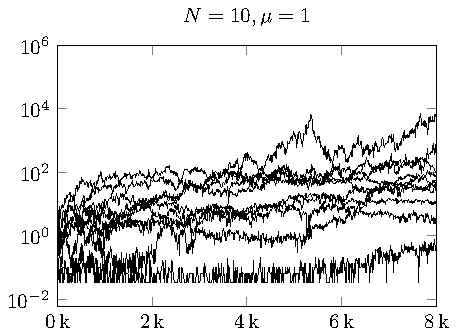
\includegraphics[scale=1]{plots/ce_ConstantNoise_l10_o1_all} &
\includegraphics[scale=1]{plots/ce_ConstantNoise_l13_o6_all} //
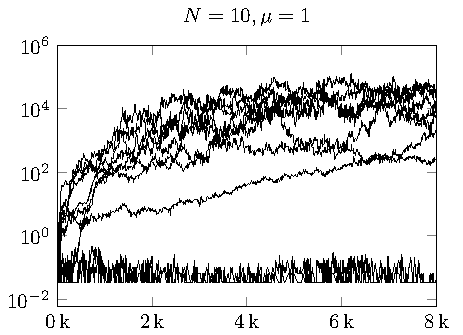
\includegraphics[scale=1]{plots/ce_ConstantNoise_l10_o5_all} &
\end{tabular}

\begin{tabular}{@{}l@{}l@{}}
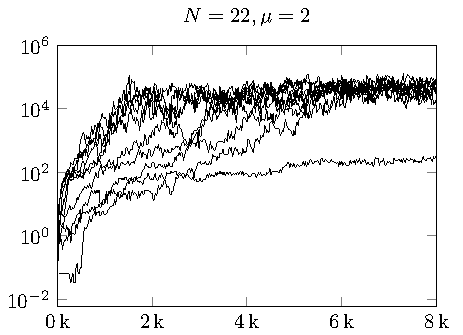
\includegraphics[scale=1]{plots/ce_ConstantNoise_l22_o2_all}&
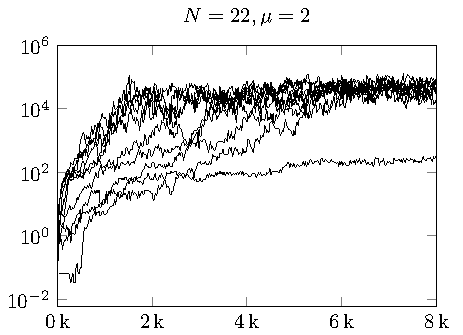
\includegraphics[scale=1]{plots/ce_ConstantNoise_l22_o2_all}
\end{tabular}

\begin{tabular}{@{}l@{}l@{}}
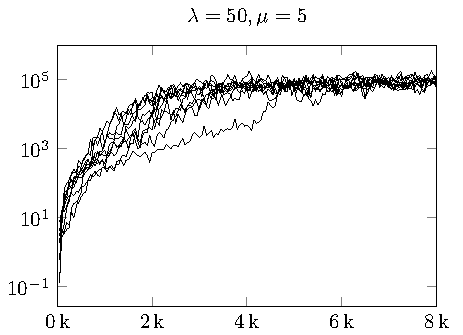
\includegraphics[scale=1]{plots/ce_ConstantNoise_l50_o5_all} &
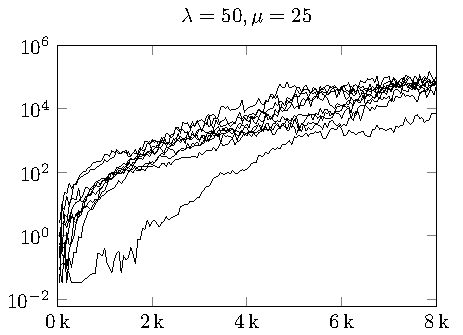
\includegraphics[scale=1]{plots/ce_ConstantNoise_l50_o25_all}
\end{tabular}

\begin{tabular}{@{}l@{}l@{}}
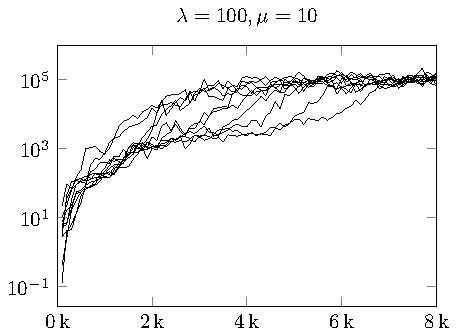
\includegraphics[scale=1]{plots/ce_ConstantNoise_l100_o10_all} &
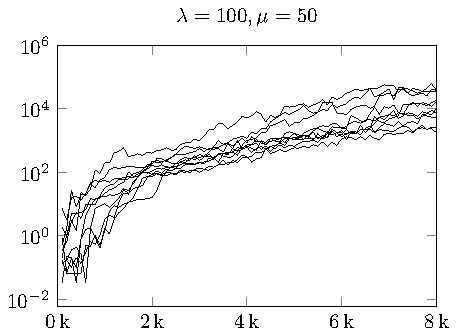
\includegraphics[scale=1]{plots/ce_ConstantNoise_l100_o50_all}
\end{tabular}

\begin{tabular}{@{}l@{}l@{}}
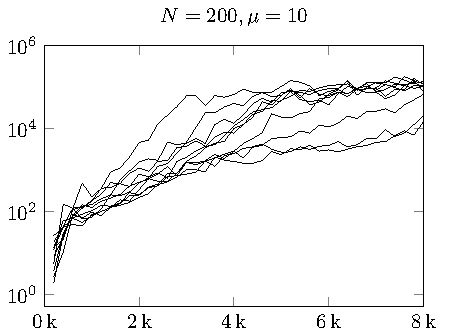
\includegraphics[scale=1]{plots/ce_ConstantNoise_l200_o20_all} &
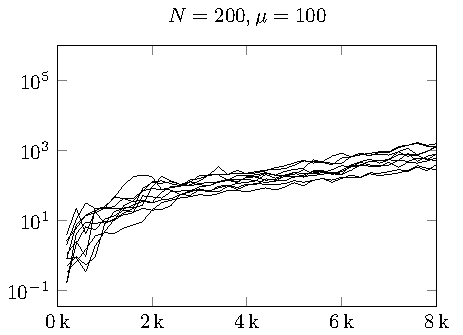
\includegraphics[scale=1]{plots/ce_ConstantNoise_l200_o100_all}
\end{tabular}





 - \comment{Insert in above section}

\clearpage

\section{Cross Entropy Implementation - Shark library}

\subsection{CrossEntropyMethod.h}

\lstinputlisting[language=c++, style=customc]{CrossEntropyMethod.h}

\clearpage

\subsection{CrossEntropyMethod.cpp}

\lstinputlisting[language=c++, style=customc]{CrossEntropyMethod.cpp}
